\documentclass[11pt]{article}
\usepackage{xcolor}
\usepackage{listings}
\usepackage{graphicx}
\usepackage{url}
\usepackage{multicol}
\usepackage{verbatim}
\usepackage{listings}
% Define a custom color for the terminal command
\definecolor{terminalcolor}{RGB}{0, 128, 0}
\definecolor{codeBackground}{rgb}{0.1,0.1,0.1}
\definecolor{codeText}{rgb}{1, 1, 1}

% Define a custom command for highlighting terminal commands
\newcommand{\terminal}[1]{\texttt{\color{terminalcolor}#1}}

\begin{document}

\begin{titlepage}
    \begin{center}
        
\includegraphics[scale=0.35]{du_logo.png}\par
        \begin{Huge}
            \textsc{University of Dhaka}\par
        \end{Huge}
        \begin{Large}
            Department of Computer Science and Engineering\par \vspace{1cm}
            CSE-3111 : Computer Networking Lab \\[12pt]    
            Lab Report 2 : Introduction to Client-Server Communication using Socket Programming Machine Operation
        \end{Large}
    \end{center}
    
    \vfill
    
    \begin{large}
        \begin{multicols}{2}
            \noindent
            \textbf{Submitted By :\\[12pt]}
                Name: Md. Emon Khan\\[8pt]
                Roll No : 30\\[12pt]
                Name: Mahmudul Hasan\\[8pt]
                Roll No : 60\\[12pt]
                
            \columnbreak
            
            \noindent
            \textbf{Submitted To :\\[12pt]}
                Dr. Md. Abdur Razzaque\\[12pt]
                Dr. Md. Mamun Or Rashid\\[12pt]
                Dr. Muhammad Ibrahim\\[12pt]
                Md. Redwan Ahmed Rizvee
        \end{multicols}    
    \end{large} 
    
\textbf{Submitted On :} February 1, 2024\\[20pt]

\end{titlepage}

\section{Introduction}
The main objective of Lab Experiment-2 is to employ socket programming for the implementation of client-server communication using the TCP protocol. Socket programming involves creating a server socket and specifying a port for communication. The client can then utilize this socket to establish a connection with the server and exchange data.

\subsection{Objectives}
The specific objectives of the lab experiment include:
\begin{itemize}
    \item Establishing client-server communication using the TCP protocol using socket programming as the fundamental goal.
    \item Testing the communication by exchanging data and performing specific operations:
    \begin{itemize}
        \item Converting a provided string from uppercase to lowercase on the client side.
        \item Sending a number to the server and instructing it to determine whether the number is prime or not, or whether it's a palindrome or not.
    \end{itemize}
    \item Implementing an ATM server, where the client sends a money exchange request.
    \item Ensuring the ATM server is capable of handling errors effectively.
\end{itemize}

\section{Theory}
    A socket serves as a software endpoint facilitating the connection between two devices for data exchange. Socket programming involves creating a listener socket (server-side) and a client socket, establishing a connection with the server for communication. This interaction can take place using protocols like TCP or UDP.
    \begin{figure}
        \centering
        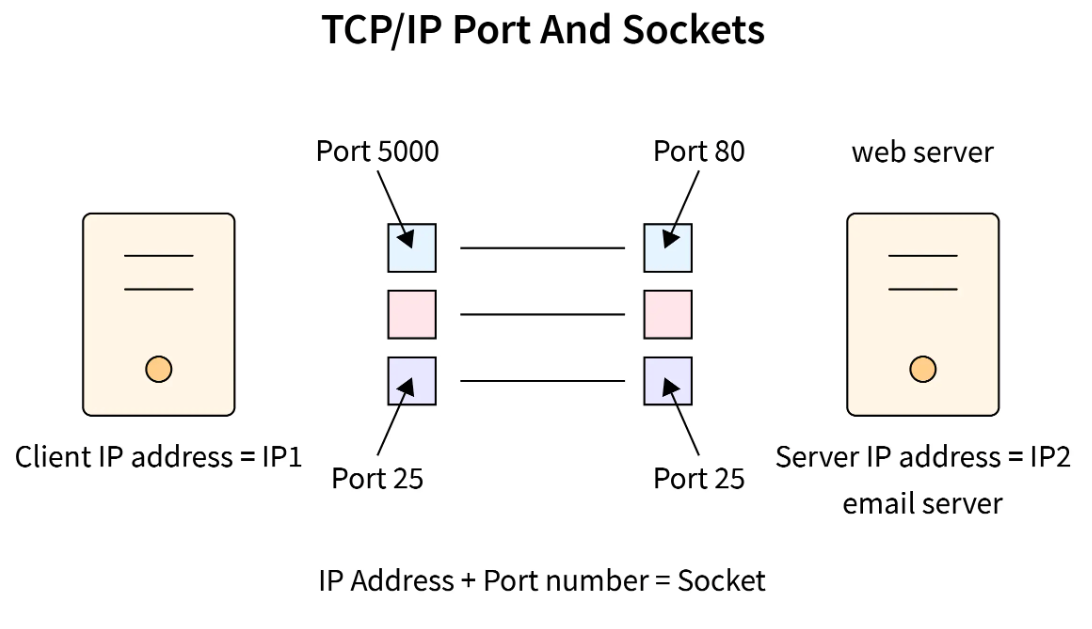
\includegraphics[width=\textwidth]{socketProgramming.png}
        \caption{Socket Programming}
        \label{fig:enter-label}
    \end{figure}

\section{Methodology}

    \subsection{Establishing a TCP connection}
        \subsubsection{Server}
        On our server side, we initiate the creation of a server socket using the TCP protocol and bind it to a specific host address along with an available port. Subsequently, we set our server in listening mode, awaiting any incoming connection requests. Once a connection request is received, we proceed to establish a connection with the client by accepting the request.
        \subsubsection{Client}
        On the client side, we initiate the creation of a client socket, also using the TCP protocol. After this, we send a connection request to the previously established server, using the host address and port.
        
    \subsection{Capital to Small Letter Conversion}
        \subsubsection{Server}
        The server awaits a request from the client. Upon reception, it decodes the expected message, which is anticipated to be a string in uppercase Latin letters. It convert the message to lowercase, encode it, and send the modified message back to the client.
        \subsubsection{Client}
        The client transmits a string of uppercase Latin letters to the server after encoding the message, and then awaits a reply. Upon receiving the server's response, the client proceeds to decode the message.
    \subsection{Prime or Palindrome Test}
        \subsubsection{Server}
        The server awaits two requests from the client. The initial request is anticipated to be a number, and the following request specifies a particular test, such as a Prime test or a Palindrome test. Upon decoding these requests, the server comprehends the specified operation, sending the number to the appropriate function. Following the function's execution, the server processes the output, and sends the relevant result encoded as a reply to the client.
        \subsubsection{Client}
        The client sends two requests to the server. The first request is expected to be a number, and the latter specifies a particular test, such as a Prime test or a Palindrome test. These requests are encoded and transmitted to the server. Then the client awaits a reply. Upon receiving the reply, it proceeds to decode the response for further processing.
    \subsection{ATM Machine}
        \subsubsection{Server}
        The server awaits two requests from the client. The initial request is anticipated to be a number, and the following request specifies a particular request, such as a Withdrawal or a Deposition. Upon decoding these requests, the server comprehends the specified operation, sending the number to the appropriate function. Following the function's execution, the server processes the output, and sends the relevant result encoded as a reply to the client.
        \subsubsection{Client}
        The client sends two requests to the server. The first request is expected to be a number, and the latter specifies a particular request, such as a Withdrawal or a Deposition. These requests are encoded and transmitted to the server. Then the client awaits a reply. Upon receiving the reply, it proceeds to decode the response for further processing.
    \subsection{Error Handling}
        \subsubsection{Server}
        The server issues a pseudo-error. When it produces an error, it doesn't get the client's request. So the server keeps on listening until it gets the client request. The client on the other hand, calculated the elapsed time from the start of the session, to the server's reply.
        \subsubsection{Client}
        The client issues a pseudo-error and halts for some time. Meanwhile the server keeps on listening. The client keeps note of the elapsed time during the whole transaction.

\newpage
\section{Experimental result}

Some Snapshots of the terminal output for each of these tools.
    \subsection{Capital to Small Conversion}
        \subsubsection{Server}
        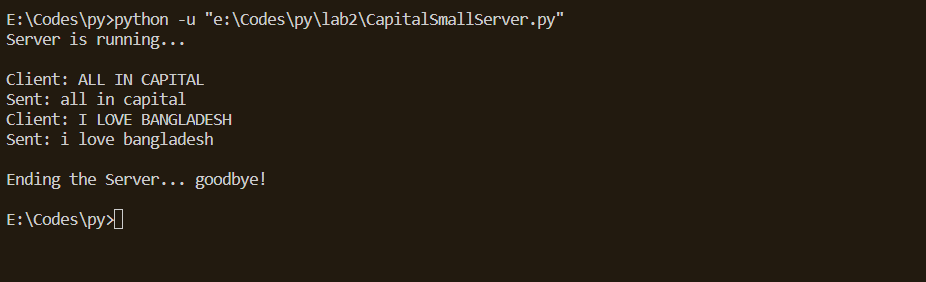
\includegraphics[width=\textwidth]{Server Capital Small.png}
        \subsubsection{Client}
        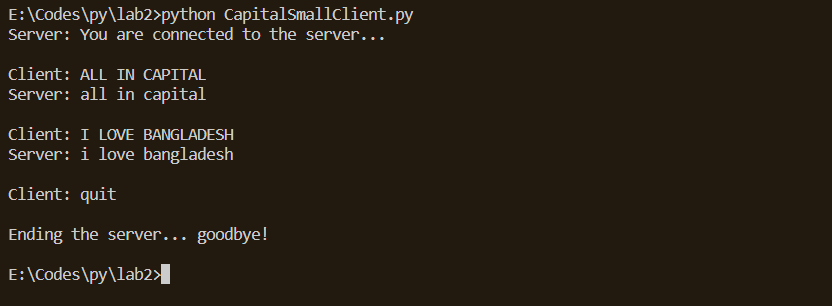
\includegraphics[width=\textwidth]{Client Capital Small.png}
    \subsection{Prime or Palindrome}
        \subsubsection{Server}
        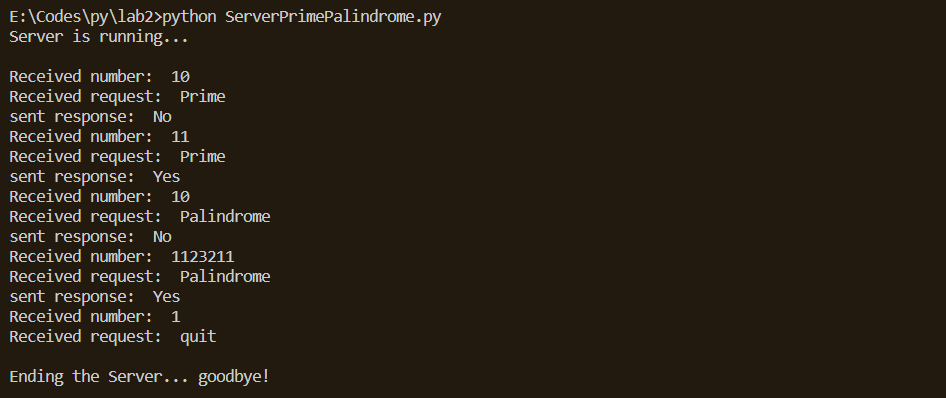
\includegraphics[width=\textwidth]{Server Prime Palindrome.png}
        \subsubsection{Client}
        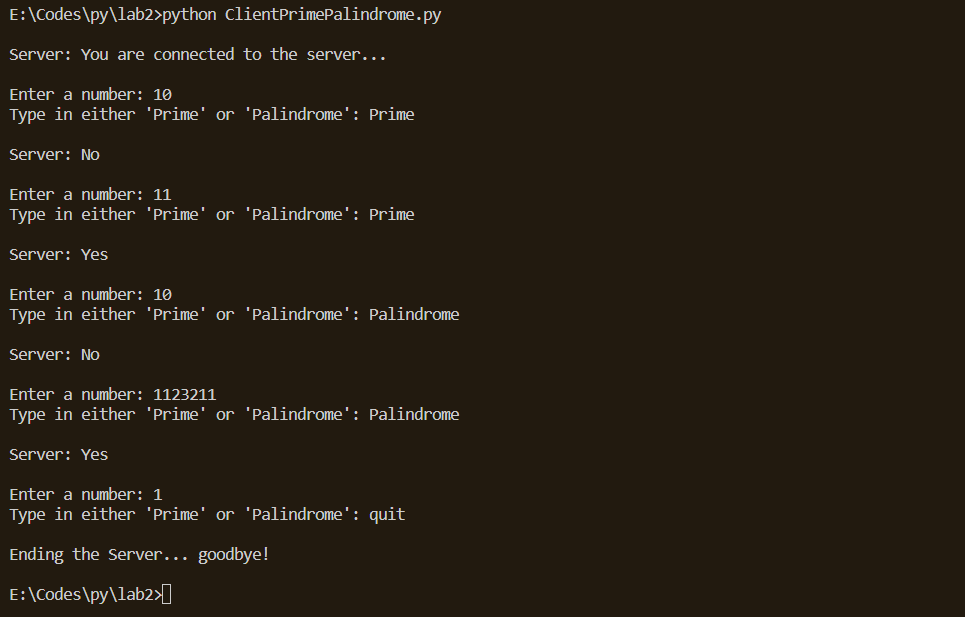
\includegraphics[width=\textwidth]{Client Prime Palindrome.png}
    \subsection{ATM Machine}
        \subsubsection{Server}
        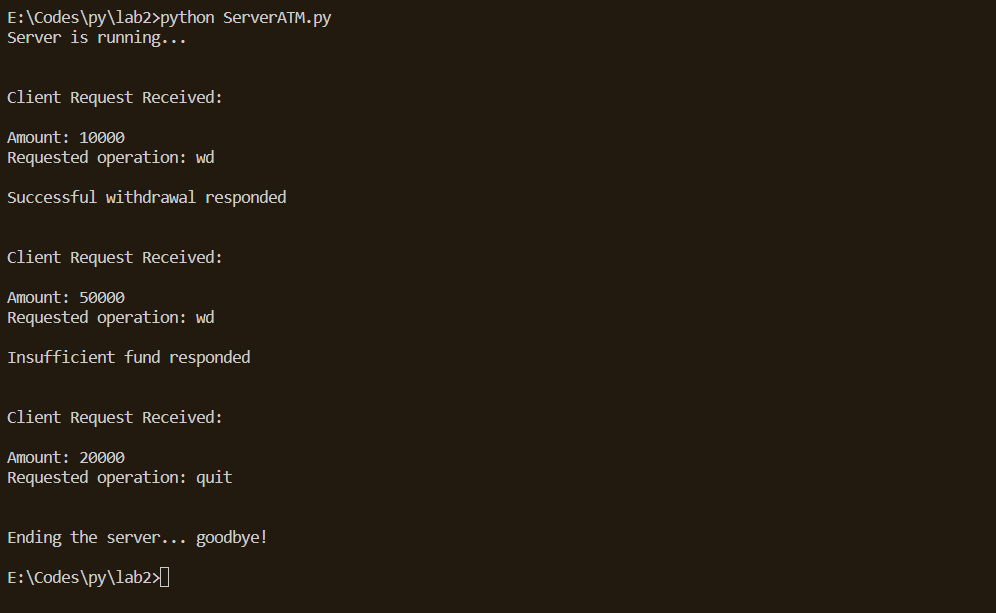
\includegraphics[width=\textwidth]{ServerATM.png}
        \subsubsection{Client}
        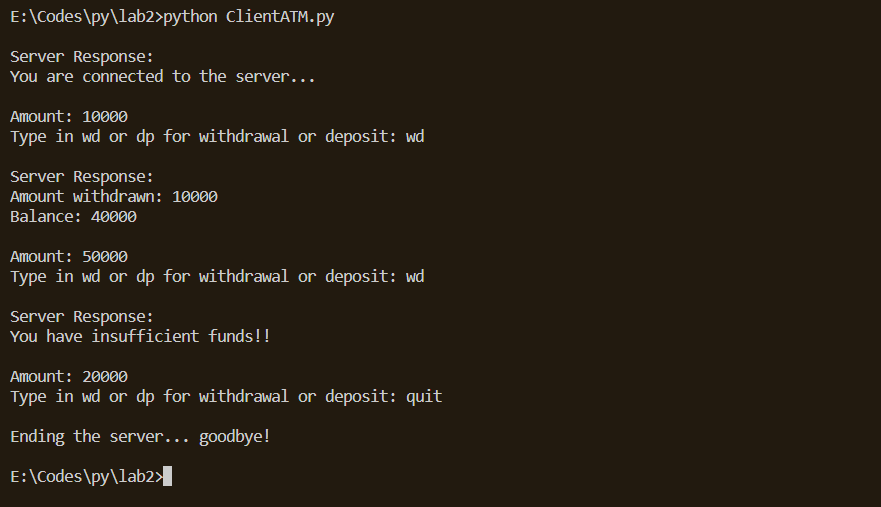
\includegraphics[width=\textwidth]{ClientATM.png}
    \subsection{ATM Machine: Error Handling}
        \subsubsection{Server}
        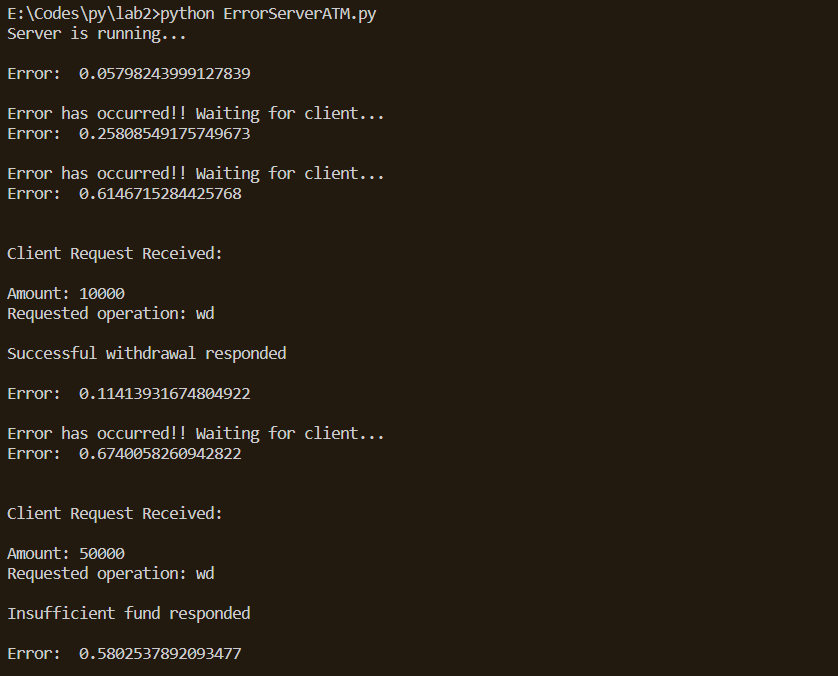
\includegraphics[width=\textwidth]{ErrorServer1.png}
        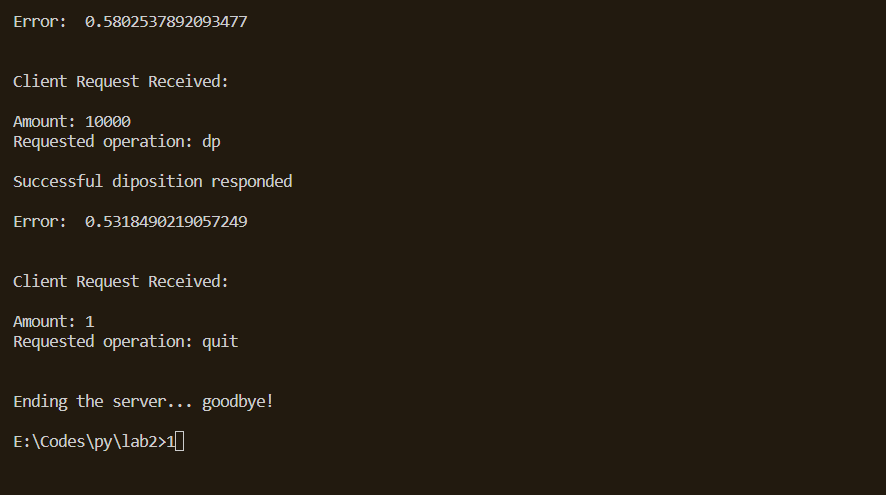
\includegraphics[width=\textwidth]{ErrorServer2.png}
        \subsubsection{Client}
        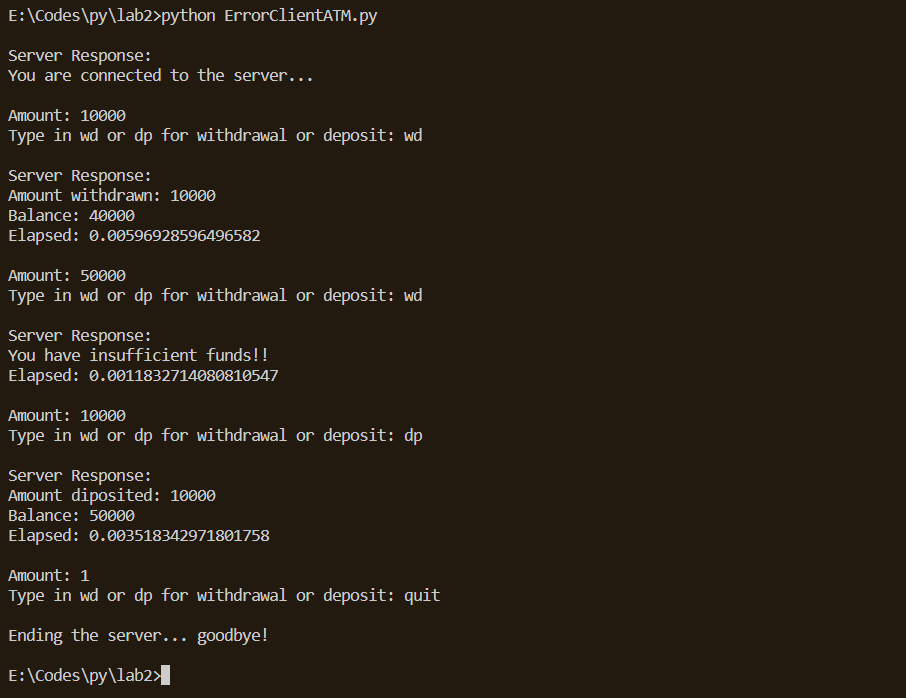
\includegraphics[width=\textwidth]{ErrorClient.png}
    \subsection{Error Analysis}
    Now in this Error handling, we used different percentages of error occurrence. Here's a graph of the response time of the server with respect to the error percentages
    
        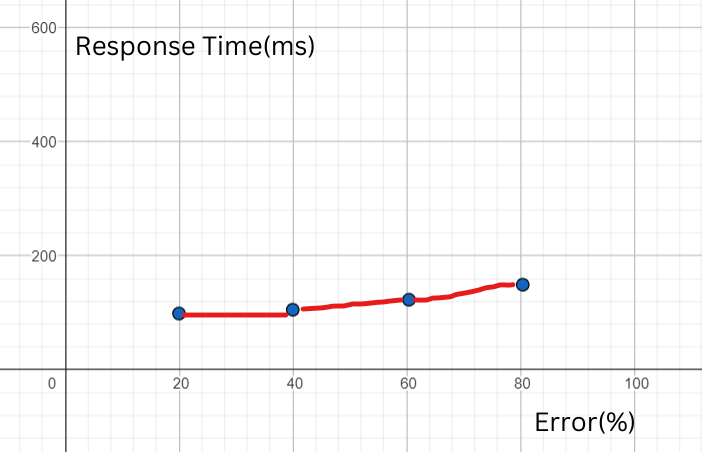
\includegraphics[width=\textwidth]{graph.png}

\section{Experience}
\begin{enumerate}
    \item We had to look up the server device IP to establish the connection
    \item We established a client-server communication between two different devices using socket programming for the first time
    \item We learned how errors are handled in a TCP connection
\end{enumerate}

\section*{Appendix}

All the codes are provided in Python programming language

\subsection*{Code for Capital to Small Conversion}
\subsubsection*{Server}
\begin{verbatim}
import socket

# HOST_IP = "10.33.2.94"
HOST_IP = socket.gethostbyname(socket.gethostname())
HOST_PORT = 12348
ENCODER = "utf-8"
BYTESIZE = 1024

server_socket = socket.socket(socket.AF_INET, socket.SOCK_STREAM)
server_socket.bind((HOST_IP, HOST_PORT))
server_socket.listen()

print("Server is running... \n")
client_socket, client_address = server_socket.accept()

client_socket.send("You are connected to the server...".encode(ENCODER))

while True:
    message = client_socket.recv(BYTESIZE).decode(ENCODER)

    if message == "quit":
        client_socket.send("quit".encode(ENCODER))
        print("\nEnding the Server... goodbye!")
        break
    else:
        print(f"Client: {message}")
        client_socket.send((message.lower()).encode(ENCODER))
        print(f"Sent: {message.lower()}")

server_socket.close()
\end{verbatim}
\subsubsection*{Client}
\begin{verbatim}
import socket

#DEST_IP = "10.33.2.94"

DEST_IP = socket.gethostbyname(socket.gethostname())
DEST_PORT = 12348
ENCODER = "utf-8"
BYTESIZE = 1024

client_socket = socket.socket(socket.AF_INET, socket.SOCK_STREAM)
client_socket.connect((DEST_IP, DEST_PORT))

while True:
    message = client_socket.recv(BYTESIZE).decode(ENCODER)

    if message == "quit":
        client_socket.send("quit".encode(ENCODER))
        print("\nEnding the server... goodbye!")
        break
    else:
        print(f"Server: {message}")
        user_input = input(f"\nClient: ")
        client_socket.send(user_input.encode(ENCODER))

client_socket.close()
\end{verbatim}

\subsection*{Code for Prime and Palindrome Test}
\subsubsection*{Server}
\begin{verbatim}
import socket

# HOST_IP = '10.33.2.94'
HOST_IP = socket.gethostbyname(socket.gethostname())
HOST_PORT = 12349
ENCODER = "utf-8"
BYTESIZE = 1024

server_socket = socket.socket(socket.AF_INET, socket.SOCK_STREAM)
server_socket.bind((HOST_IP, HOST_PORT))
server_socket.listen()

print("Server is running... \n")
client_socket, client_address = server_socket.accept()

client_socket.send("You are connected to the server...".encode(ENCODER))

def isPrime(n):
    if n < 2:
        return "No"
    i = 2
    while i*i <= n:
        if n%i == 0:
            return "No"
        i += 1
    return "Yes"

def isPalindrome(n):
    if n == n[::-1]:
        return "Yes"
    return "No"

while True:
    number = client_socket.recv(BYTESIZE).decode(ENCODER)
    print("Received number: ", number)
    op = client_socket.recv(BYTESIZE).decode(ENCODER)
    print("Received request: ", op)

    if op == "quit":
        client_socket.send("quit".encode(ENCODER))
        print("\nEnding the Server... goodbye!")
        break
    elif op == 'Prime':
        message = isPrime(int(number))
        client_socket.send(message.encode(ENCODER))
        print("sent response: ", message)
    elif op == "Palindrome":
        message = isPalindrome(number)
        client_socket.send(message.encode(ENCODER))
        print("sent response: ", message)

server_socket.close()
\end{verbatim}
\subsubsection*{Client}
\begin{verbatim}
import socket

# HOST_IP = '10.33.2.94'
DEST_IP = socket.gethostbyname(socket.gethostname())
DEST_PORT = 12349
ENCODER = "utf-8"
BYTESIZE = 1024

client_socket = socket.socket(socket.AF_INET, socket.SOCK_STREAM)
client_socket.connect((DEST_IP, DEST_PORT))

while True:
    message = client_socket.recv(BYTESIZE).decode(ENCODER)

    if message == "quit":
        client_socket.send("quit".encode(ENCODER))
        print("\nEnding the Server... goodbye!")
        break
    else:
        print(f"\nServer: {message}")
        user_input = input(f"\nEnter a number: ")
        client_socket.send(user_input.encode(ENCODER))
        user_input = input(f"Type in either 'Prime' or 'Palindrome': ")
        client_socket.send(user_input.encode(ENCODER))

client_socket.close()
\end{verbatim}

\subsection*{Code for ATM Server Implementation}
\subsubsection*{Server}
\begin{verbatim}
import socket

# HOST_IP = '10.33.2.94'
HOST_IP = socket.gethostbyname(socket.gethostname())
HOST_PORT = 12348
ENCODER = "utf-8"
BYTESIZE = 1024

server_socket = socket.socket(socket.AF_INET, socket.SOCK_STREAM)
server_socket.bind((HOST_IP, HOST_PORT))
server_socket.listen()

print("Server is running... \n")
client_socket, client_address = server_socket.accept()

client_socket.send("You are connected to the server...".encode(ENCODER))

balance = 50000

while True:
    amount = client_socket.recv(BYTESIZE).decode(ENCODER)
    print('\nClient Request Received:\n')
    print(f'Amount: {amount}')
    op = client_socket.recv(BYTESIZE).decode(ENCODER)
    print(f'Requested operation: {op}\n')

    if op == "quit":
        client_socket.send("quit".encode(ENCODER))
        print("\nEnding the server... goodbye!")
        break
    elif op == 'wd':
        if balance < int(amount):
            client_socket.send("You have insufficient funds!!".encode(ENCODER))
            print('Insufficient fund responded\n')
        else:
            balance -= int(amount)
            response = "Amount withdrawn: " + str(amount) + "\nBalance: " + str(balance)
            client_socket.send(response.encode(ENCODER))
            print('Successful withdrawal responded\n')
    elif op == 'dp':
        balance += int(amount)
        response = "Amount diposited: " + str(amount) + "\nBalance: " + str(balance)
        client_socket.send(response.encode(ENCODER))
        print('Successful diposition responded\n')
server_socket.close()
\end{verbatim}
\subsubsection*{Client}
\begin{verbatim}
import socket

DEST_IP = socket.gethostbyname(socket.gethostname())

# DEST_IP = '10.33.2.94'
DEST_PORT = 12348
ENCODER = "utf-8"
BYTESIZE = 1024

client_socket = socket.socket(socket.AF_INET, socket.SOCK_STREAM)
client_socket.connect((DEST_IP, DEST_PORT))

while True:
    message = client_socket.recv(BYTESIZE).decode(ENCODER)

    if message == "quit":
        client_socket.send("quit".encode(ENCODER))
        print("\nEnding the server... goodbye!")
        break
    else:
        print(f"\nServer Response:\n{message}")
        user_input = input("\nAmount: ")
        client_socket.send(user_input.encode(ENCODER))
        user_input = input("Type in wd or dp for withdrawal or deposit: ")
        client_socket.send(user_input.encode(ENCODER))

client_socket.close()
\end{verbatim}
\subsection*{Code for Error Handling in ATM server}
\subsubsection*{Server}
\begin{verbatim}
import socket
import random
import time

# HOST_IP = '10.33.2.94'
HOST_IP = socket.gethostbyname(socket.gethostname())
HOST_PORT = 12348
ENCODER = "utf-8"
BYTESIZE = 1024

server_socket = socket.socket(socket.AF_INET, socket.SOCK_STREAM)
server_socket.bind((HOST_IP, HOST_PORT))
server_socket.listen()

print("Server is running... \n")
client_socket, client_address = server_socket.accept()

client_socket.send("You are connected to the server...".encode(ENCODER))

errorPercentage = 0.2           #or whatever error percetage
balance = 50000

while True:
    error = random.random()
    print("Error: ", error, "\n")

    if error <= errorPercentage:
        print('Error has occurred!! Waiting for client...')
    else:
        amount = client_socket.recv(BYTESIZE).decode(ENCODER)
        print('\nClient Request Received:\n')
        print(f'Amount: {amount}')
        op = client_socket.recv(BYTESIZE).decode(ENCODER)
        print(f'Requested operation: {op}\n')
        if op == 'quit':
            client_socket.send('quit'.encode(ENCODER))
            print("\nEnding the server... goodbye!")
            break
        elif op == 'wd':
            if balance < int(amount):
                client_socket.send("You have insufficient funds!!".encode(ENCODER))
                print('Insufficient fund responded\n')
            else:
                balance -= int(amount)
                response = "Amount withdrawn: " + str(amount) + "\nBalance: " + str(balance)
                client_socket.send(response.encode(ENCODER))
                print('Successful withdrawal responded\n')
        elif op == 'dp':
            balance += int(amount)
            response = "Amount diposited: " + str(amount) + "\nBalance: " + str(balance)
            client_socket.send(response.encode(ENCODER))
            print('Successful diposition responded\n')

server_socket.close()
\end{verbatim}
\subsubsection*{Client}
\begin{verbatim}
import socket
import time

DEST_IP = socket.gethostbyname(socket.gethostname())

# DEST_IP = '10.33.2.94'
DEST_PORT = 12348
ENCODER = "utf-8"
BYTESIZE = 1024

client_socket = socket.socket(socket.AF_INET, socket.SOCK_STREAM)
client_socket.connect((DEST_IP, DEST_PORT))

amount = "0"
opcode = "dp"

start_time = time.time()
end_time = time.time()

requested = False

while True:
    message = client_socket.recv(BYTESIZE).decode(ENCODER)
    if message.lower() == "quit":
        client_socket.send("quit".encode(ENCODER))
        print("\nEnding the server... goodbye!")
        break
    else:
        print(f"\nServer Response:\n{message}")

        if requested:
            end_time = time.time()
            elapsed_time = end_time - start_time
            print(f"Elapsed: {elapsed_time}")
        
        amount = input("\nAmount: ")
        client_socket.send(amount.encode(ENCODER))
        opcode = input("Type in wd or dp for withdrawal or deposit: ")
        client_socket.send(opcode.encode(ENCODER))
        requested = True
        start_time = time.time()

client_socket.close()
\end{verbatim}

\begin{thebibliography}{1}
    \bibitem{Real Python} \url{https://realpython.com/}
    \bibitem{Geeks For Geeks} \url{https://www.geeksforgeeks.org/}
    \bibitem{Morioh Blog} \url{https://morioh.com/}
\end{thebibliography}

\end{document}
